\section{Az egyenáramú motor diszkrét idejű modellezése}
Ebben a feladatban csak a motort vizsgálom hajtómű és tárcsa nélkül ($\Delta t = 0.040$ s).
\subsection{a) Folytonos idejű állapottér modell}
Az állapottér modell változói $\mathbf{x} = [i \quad \omega]^\top$. A differenciálegyenletek alapján az átírási forma $\mathbf{\dot{x}} = \mathbf{A} \mathbf{x} + \mathbf{B} u$:
\begin{equation}
\mathbf{A} = 
\begin{bmatrix}
-\frac{R}{L} & -\frac{k_m}{L} \\
\frac{k_m}{J_r} & -\frac{B}{J_r}
\end{bmatrix}
=
\begin{bmatrix}
-10052.6 & -21.1 \\
31825.4 & -1.587
\end{bmatrix}
\end{equation}
\begin{equation}
\mathbf{B} = 
\begin{bmatrix}
\frac{1}{L} \\
0
\end{bmatrix}
=
\begin{bmatrix}
526.31 \\
0
\end{bmatrix}
\end{equation}
$\mathbf{C} = \begin{bmatrix} 0 & 1 \end{bmatrix}$, $\mathbf{D} = 0$.

\subsection{b) Előretartó (forward) Euler modell}
A diszkretizált állapottér egyenletek előretartó Euler módszerrel:
\begin{equation}
\mathbf{x}_{k+1} = (\mathbf{I} + \mathbf{A}\Delta t) \mathbf{x}_k + (\mathbf{B}\Delta t) u_k = \mathbf{A}_{de} \mathbf{x}_k + \mathbf{B}_{de} u_k
\end{equation}
\begin{equation}
\mathbf{A}_{de} = 
\begin{bmatrix}
-401.1 & -0.844 \\
1273.0 & 0.936
\end{bmatrix}, \quad
\mathbf{B}_{de} = 
\begin{bmatrix}
21.05 \\
0
\end{bmatrix}
\end{equation}

\subsection{c) Hátratartó (backward) Euler modell}
A hátratartó Euler módszer diszkretizációs formulája:
\begin{equation}
\mathbf{A}_{dh} = (\mathbf{I} - \mathbf{A}\Delta t)^{-1} = 
\begin{bmatrix}
7.07 \cdot 10^{-4} & -5.61 \cdot 10^{-4} \\
0.8467 & 0.2681
\end{bmatrix}
\end{equation}
\begin{equation}
\mathbf{B}_{dh} = \mathbf{A}_{dh} \mathbf{B} \Delta t = 
\begin{bmatrix}
0.01489 \\
17.8265
\end{bmatrix}
\end{equation}

\subsection{d) A diszkrét és folytonos modellek viselkedése}
\begin{figure}[H]
    \centering
    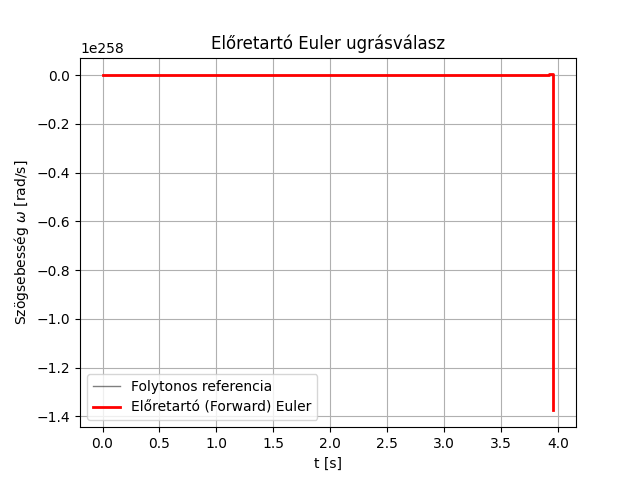
\includegraphics[width=0.7\textwidth]{res/imgs/fig_EulerElore.png}
    \caption{Előretartó Euler ($T=0.04$ s).}
\end{figure}
\begin{figure}[H]
    \centering
    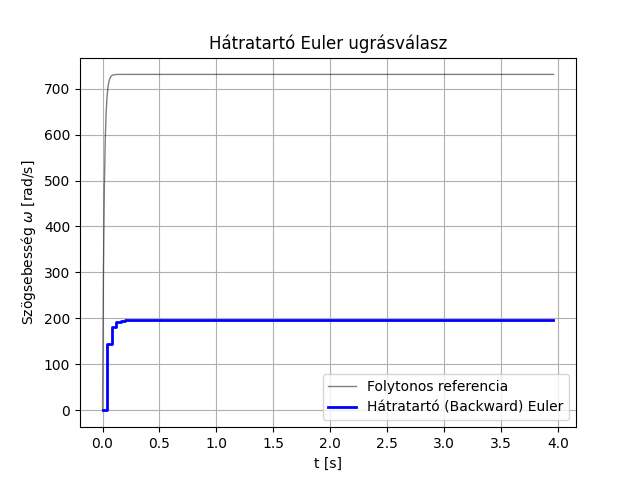
\includegraphics[width=0.7\textwidth]{res/imgs/fig_EulerHatra.png}
    \caption{Hátratartó Euler ($T=0.04$ s).}
\end{figure}
A vizsgálat során megfigyelhető, hogy a $0.040$ s-os lépésköz túlságosan nagy a rendszer domináns időállandójához képest ($\approx 0.1$ ms). Ennek következtében az előretartó Euler módszer durván instabillá válik. A hátratartó Euler módszer stabilitását megőrzi a módszer sajátosságai miatt, azonban jelentős csillapítást visz a rendszerbe emiatt eltorzítja az átmenetet.
